\documentclass{article}
\usepackage[letterpaper]{geometry}
\geometry{verbose,tmargin=1in,bmargin=1in,lmargin=1in,rmargin=1in}

\usepackage[utf8]{inputenc}
\usepackage{amsmath}
\usepackage{amssymb}
\usepackage{listings}
\usepackage{graphicx}
\usepackage{enumitem}
\usepackage{caption}
\usepackage{subcaption}

\title{CIS 419/519: Homework 3}
\author{Jiatong Sun}
\date{}

\begin{document}
    \maketitle
	Although the solutions are entirely my own, I consulted with the following people and sources while working on this homework: $Junfan Pan$
    
    \section{Logistic Regression}
    	\begin{enumerate}
    	\item [1.3]Analysis
    	
    	\begin{figure}[h!]
     	\centering
     	\begin{subfigure}[b]{0.44\textwidth}
         	\centering
         	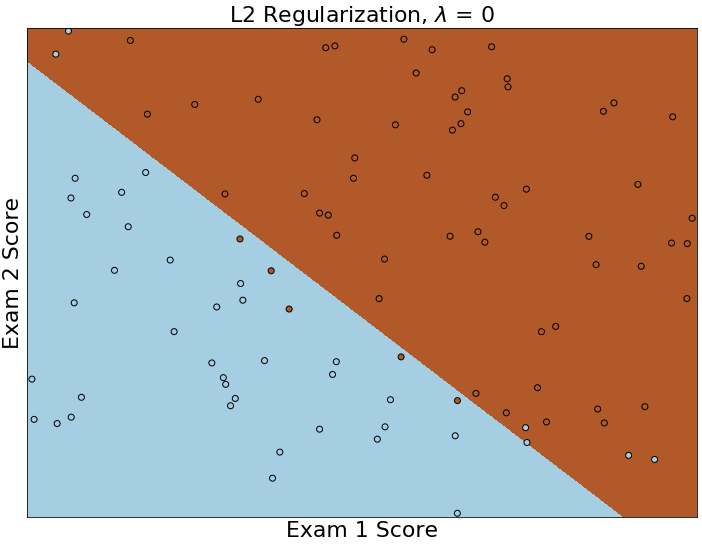
\includegraphics[width=\textwidth]
         	{Problem_1_3/fig_L2_1.png}
         	\caption{$\lambda = 0, regNorm = 2$}
         	\label{fig:L2_1}
     	\end{subfigure}
     	\hfill
     	\begin{subfigure}[b]{0.44\textwidth}
         	\centering
         	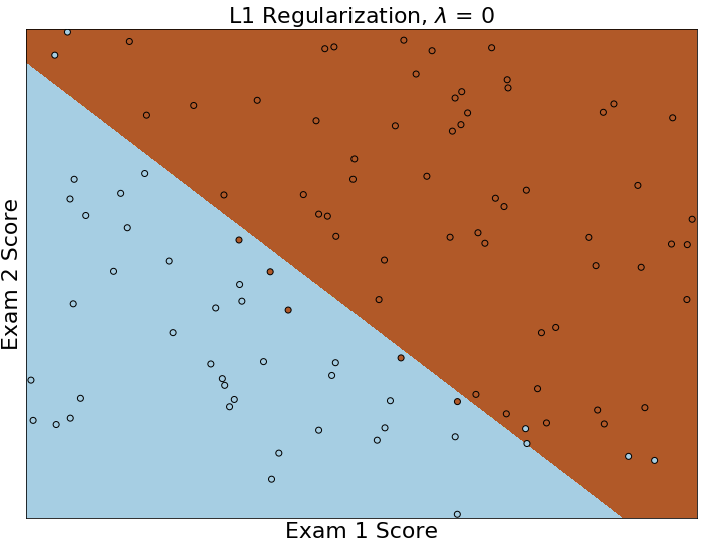
\includegraphics[width=\textwidth]
         	{Problem_1_3/fig_L1_1.png}
         	\caption{$\lambda = 0, regNorm = 1$}
         	\label{fig:L1_1}
     	\end{subfigure}
		\end{figure}
		
    	\begin{figure}[h!]
     	\centering
     	\begin{subfigure}[b]{0.44\textwidth}
         	\centering
         	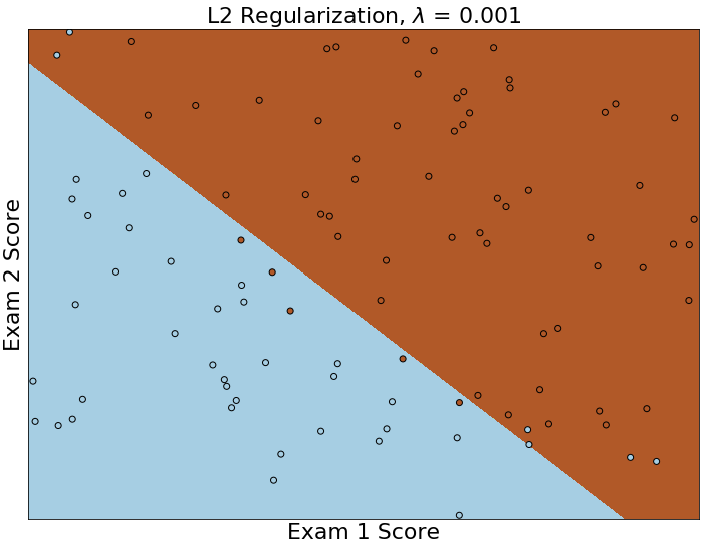
\includegraphics[width=\textwidth]
         	{Problem_1_3/fig_L2_2.png}
         	\caption{$\lambda = 0.001, regNorm = 2$}
         	\label{fig:L2_2}
     	\end{subfigure}
     	\hfill
     	\begin{subfigure}[b]{0.44\textwidth}
         	\centering
         	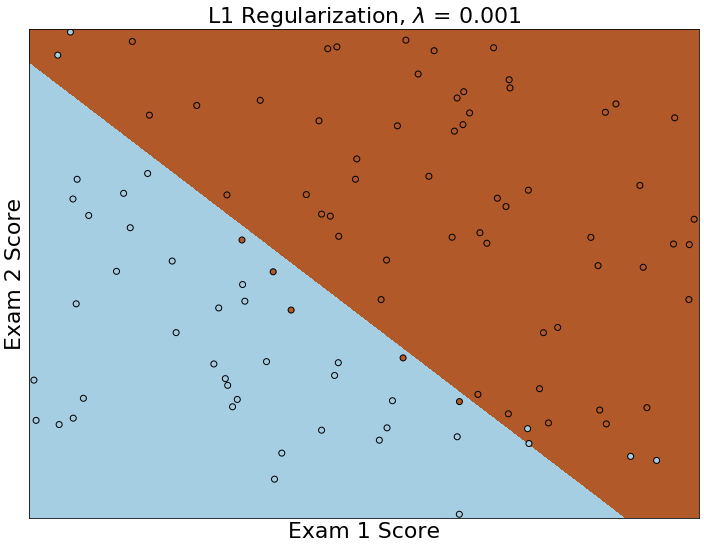
\includegraphics[width=\textwidth]
         	{Problem_1_3/fig_L1_2.png}
         	\caption{$\lambda = 0.001, regNorm = 1$}
         	\label{fig:L1_2}
     	\end{subfigure}
		\end{figure}
		
    	\begin{figure}[h!]
     	\centering
     	\begin{subfigure}[b]{0.44\textwidth}
         	\centering
         	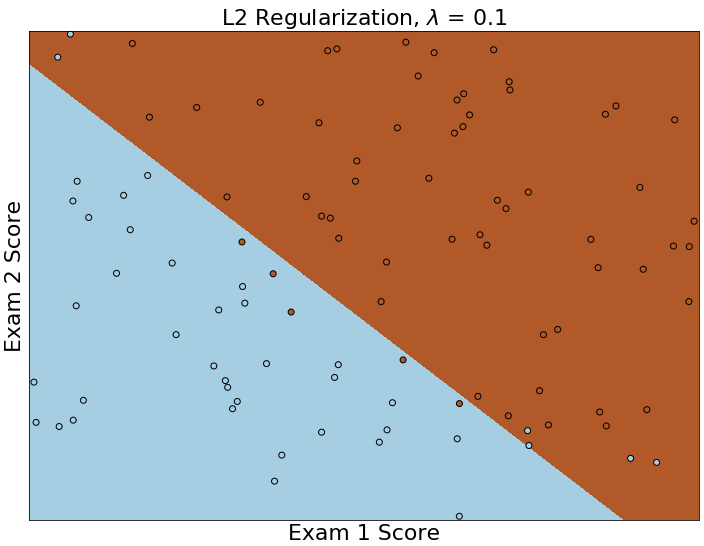
\includegraphics[width=\textwidth]
         	{Problem_1_3/fig_L2_3.png}
         	\caption{$\lambda = 0.1, regNorm = 2$}
         	\label{fig:L2_3}
     	\end{subfigure}
     	\hfill
     	\begin{subfigure}[b]{0.44\textwidth}
         	\centering
         	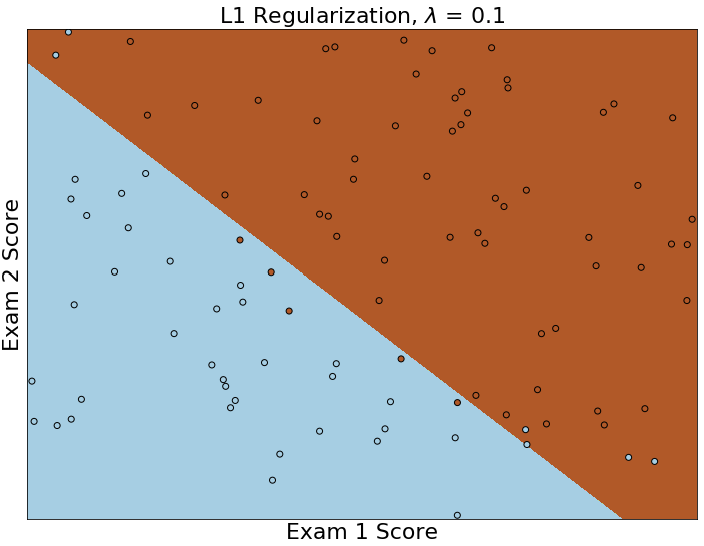
\includegraphics[width=\textwidth]
         	{Problem_1_3/fig_L1_3.png}
         	\caption{$\lambda = 0.1, regNorm = 1$}
         	\label{fig:L1_3}
     	\end{subfigure}
		\end{figure}
		
    	\begin{figure}[h!]
     	\centering
     	\begin{subfigure}[b]{0.44\textwidth}
         	\centering
         	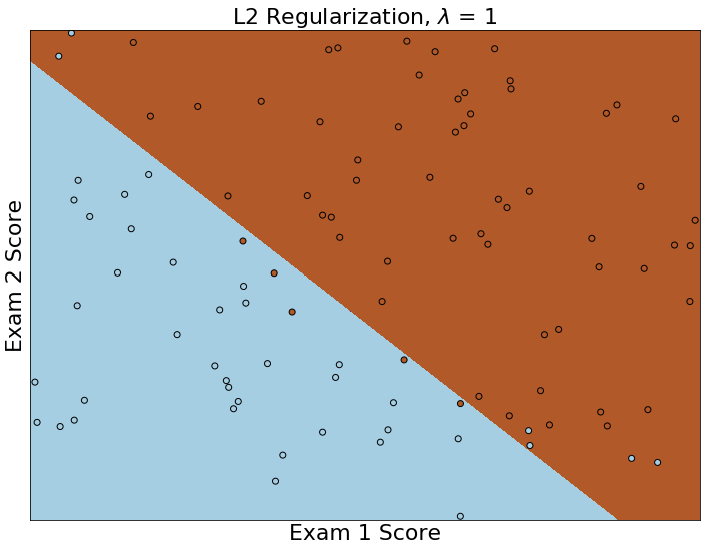
\includegraphics[width=\textwidth]
         	{Problem_1_3/fig_L2_4.png}
         	\caption{$\lambda = 1, regNorm = 2$}
         	\label{fig:L2_4}
     	\end{subfigure}
     	\hfill
     	\begin{subfigure}[b]{0.44\textwidth}
         	\centering
         	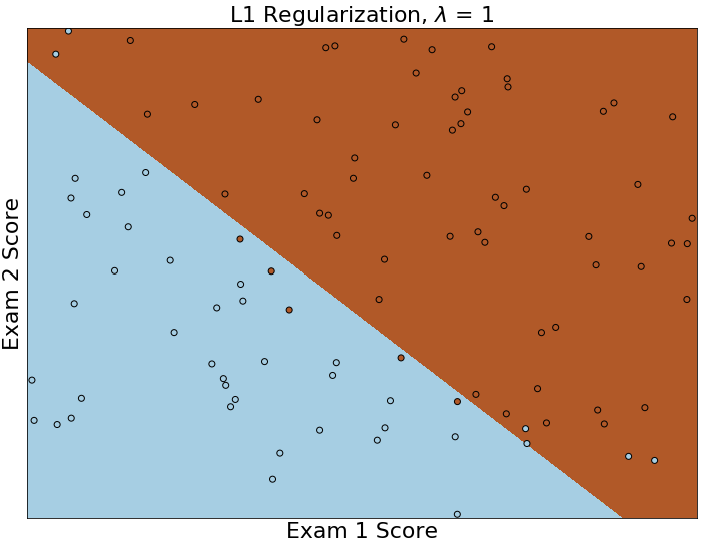
\includegraphics[width=\textwidth]
         	{Problem_1_3/fig_L1_4.png}
         	\caption{$\lambda = 1, regNorm = 1$}
         	\label{fig:L1_4}
     	\end{subfigure}
		\end{figure}
		
    	\begin{figure}[h!]
     	\centering
     	\begin{subfigure}[b]{0.44\textwidth}
         	\centering
         	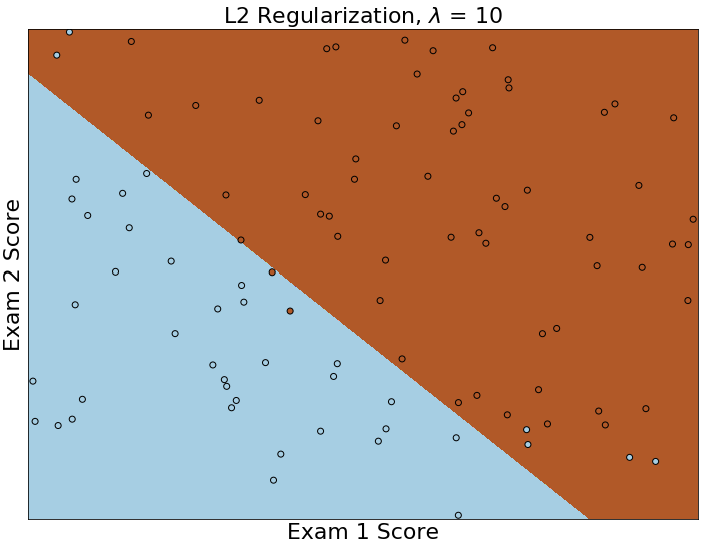
\includegraphics[width=\textwidth]
         	{Problem_1_3/fig_L2_5.png}
         	\caption{$\lambda = 10, regNorm = 2$}
         	\label{fig:L2_5}
     	\end{subfigure}
     	\hfill
     	\begin{subfigure}[b]{0.44\textwidth}
         	\centering
         	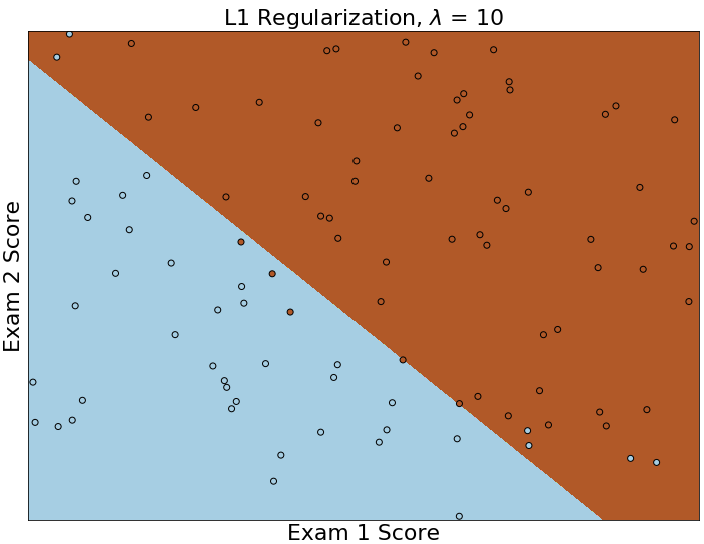
\includegraphics[width=\textwidth]
         	{Problem_1_3/fig_L1_5.png}
         	\caption{$\lambda = 10, regNorm = 1$}
         	\label{fig:L1_5}
     	\end{subfigure}
		\end{figure}
		
    	\end{enumerate}

	\newpage
	\noindent
	\textbf{Conclusion: }\\
	As the $\lambda$ increases, the border slightly moves to bottom left corner, which means more data are recognized as 1. This is because a bigger $\lambda$ causes the regularization term to be bigger and the convergence to be more quick, and thus the boarder stops moving at a relatively small iteration number. For l1 and L2, when $\lambda$ is small, the difference is hard to observe; but when $\lambda$ is greater than 1, L2 norm converges more quickly than L1 norm and thus its boarder is more close to the bottom left corner.
	
	
	
	
    \section{Comparing Algorithms} 
    	\begin{enumerate}
    	\item [2.2]Comparing Algorithms
    	
    	
    	\end{enumerate}
        
        
        
\end{document}